\section{Performance Study}

\subsection{Experimental Setup}

\textbf{Dataset.}
We divide the 124 high-school students' posts in the case study in Section 3 into two parts.
For each grade, the first training part covers the former 60\% period for each student,
and the second testing part covers the latter 40\% period.
%The first training part covers the period of
%January 1, 2012 to February 1, 2014, and the second testing part covers the period of
%March 2, 2014 to February 1, 2015.
There are 12,139 posts in the first part, and 17,093 posts in the second part.

\textbf{Ground truth.}
The 122 stressful study-related events with their duration published in the agenda of Taicang High School on its official website
are taken as the ground truth for the analysis of detected stressful periods and stressors.
Due to the continuity of human's emotion, we add a $\Delta_t$-day on either side of an event period,
based on the significance of the event and event duration (shown in Table~\ref{tab:schoolEventSummary}).
In the experiment, we set $\Delta_t$=$Sigificance$*$Duration$.
If two events overlap temporally, we collapse them into one.
From the training data, we derive $\lambda_0$
(the stressful posting rate during historic non-stressor-event periods) for each teen, and apply it
to detect maximal stressful periods and stressor events on the teen's testing data.

\textbf{Metrics.}
We evaluate the detection performance of maximal stressful periods and stressor events
through $precision$, $recall$, and the weighted average performance of precision and recall
$F_1$-$measure$, where $F_1$-$measure$=2*$precision$*$recall$/($precision$+$recall$).
%\small${Precision=TP/(TP+FP)}$ and \small${Recall=TP/(TP+FN)}$.

If a detected maximal stressful period overlaps with a study-related event period in the ground truth,
we count this detection result correctly.
We evaluate our detected stressor events from all the correctly identified maximal stressful periods.
If a stressor event in the \emph{school life} dimension is returned and ranked within the top-1/top-3 result list,
we count this event detection correctly.


\subsection{Experiment Results}
Applying the stress detection function~\cite{HIS} to each post,
we firstly sense the stress level in the category of school life, family life, peer relation, self-cognition and romantic-relation.
We then discover maximal stressful periods and rank stressor events within each maximal stressful period.

\subsubsection{Detection of Maximal Stressful Periods}

As the ground truth includes only school life related events,
we drop out detected maximal stressful periods whose stressors are not in the \emph{school life} dimension.

Fig.~\ref{fig:res_period} shows the average stressful period detection performance under different confidence thresholds $\tau$s.
When $\tau$ is less than 0.5, the recall is stable, and around 0.8 on average for the three grades students.
It starts to drop after $\tau$$>$0.5.
This is because a higher $\tau$ poses a more strict requirement on the stressful posting rate
during stressor event periods.
On the contrary, the precision increases greatly along with $\tau$ till 0.5, remains relatively stable around 0.745 until $\tau$=0.6,
and then decreases.
This verifies the statistical model that through the difference of stressful posting rates during stressor and non-stressor event periods,
we can distinguish the stressful and non-stressful periods.
When $\tau$ is around 0.59, we can achieve the highest $F_1$-$measure$ 0.734.

Comparing different grades of students, we find that the average detection performance
on Grade 3's students is the best, as illustrated in
Table~\ref{tab:PeriodPerformance}.
This might be because Grade 3 faces the strongest stress due to the final college entrance examination
than Grade 1 and 2. In its training and testing data sets, the number of scheduled stressor events and stressful periods is the most,
leading to the best result.

Another interesting observation we made is that the precision rate is less than the recall rate.
This is due to the fact that the ground truth contains only various examination events.
However, some other stressful periods like ``\emph{Having too much homework}" in the \emph{school life} dimension
are also returned, as the school normally assigns a lot more homework to its students before an exam.
As these periods do not exist in the ground truth, they are regarded as wrong results,
negatively influencing the detection precision.

\begin{figure}
\begin{minipage}{0.4\linewidth}
        \includegraphics[scale=0.38]{figs/experiment_fig/rec_period.eps}
        \centering{{\scriptsize \text{$(a)$ recall}}}
\end{minipage}
\begin{minipage}{0.6\linewidth}
    \includegraphics[scale=0.38]{figs/experiment_fig/pre_period.eps}
    \centering{{\scriptsize \text{$(b)$ precision}}}
 \end{minipage}
\caption{Performance of detected maximal stressful periods for the 124 students in three different grades.}
\label{fig:res_period}
\end{figure}

\begin{table}
\begin{center}
\caption{Performance of detecting maximal stressful periods ($\tau$=0.59)}
\begin{tabular}{|c|c|c|c|} \hline
& \textbf{Recall} & \textbf{Precision} & \textbf{$F_1$-Measure} \\ \hline
Grade 1 & 0.707 &0.705&0.706\\ \hline
Grade 2 & 0.738 &0.726&0.711\\ \hline
Grade 3 & 0.838 &0.778 &0.784\\ \hline
Average & 0.761 &0.737 &0.734\\ \hline
\end{tabular}
\label{tab:PeriodPerformance}
\end{center}
\end{table}

\subsubsection{Identification of Stressor Events}

The performance of stressor events detection exhibits a similar trend as that of stressful periods detection, as shown in
Fig.~\ref{fig:res_stressor}.
When $\tau$ is around 0.56, the highest $F_1$-$measure$ 0.759 can be obtained.
Table~\ref{tab:EventPerformance} compares the performance when we require the extracted stressor event is top-1 or top-3 ranked
in the identified maximal stressful period.
As the former is more strict, its $F_1$-Measure performance is 14.4\% less than the later one's,
mainly caused by the 8.59\% decrease of the recall.

\begin{figure}
\begin{minipage}{0.4\linewidth}
        \includegraphics[scale=0.38]{figs/experiment_fig/rec_stressor.eps}
        \centering{{\scriptsize \text{$(a)$ recall}}}
\end{minipage}
\begin{minipage}{0.5\linewidth}
    \includegraphics[scale=0.38]{figs/experiment_fig/pre_stressor.eps}
    \centering{{\scriptsize \text{$(b)$ precision}}}
 \end{minipage}
\caption{Performance of detected stressor events (in top-3 rank) for the 124 students in three different grades.}
\label{fig:res_stressor}
\end{figure}

{\footnotesize
\begin{table}
\begin{center}
\caption{Performance of detecting stressor events ($\tau$=0.56)}
\begin{footnotesize}
\begin{tabular}{|c|c|c|c|c|c|c|} \hline
\multirow{2}{1cm}{}&\multicolumn{3}{c|}{\textbf{Top-1}}&\multicolumn{3}{c|}{\textbf{Top-3}}\\\cline{2-7}
    &\textbf{Recall}&\textbf{Precision}&\textbf{$F_1$-Measure}&\textbf{Recall}&\textbf{Precision} &\textbf{$F_1$-Measure}\\\hline
Grade1  & 0.608 & 0.723 & 0.661 & 0.711 & 0.746 &0.728\\\hline
Grade2	& 0.671 & 0.69 & 0.680 & 0.745 & 0.715 &0.731\\\hline
Grade3	& 0.722	& 0.76	& 0.741 & 0.831 & 0.806 &0.818\\\hline
Average & 0.667 & 0.724 & 0.694 & 0.763 & 0.756 &0.759\\\hline
\end{tabular}
\end{footnotesize}
\label{tab:EventPerformance}
\end{center}
\end{table}
}

{\footnotesize
\begin{table}
\begin{center}
\caption{Comparison of the linguistics-based stressor event extraction method with the statistics-based life event detection approach}
\begin{footnotesize}
\begin{tabular}{|c|c|c|c|c|c|c|} \hline
\multirow{2}{1cm}{}&\multicolumn{3}{c|}{\textbf{Stressor Event Extraction (Top-1)}}&\multicolumn{3}{c|}{\textbf{Life Event Detection}}\\\cline{2-7}
    &\textbf{Recall}&\textbf{Precision}&\textbf{$F_1$-Measure}&\textbf{Recall}&\textbf{Precision}
    &\textbf{$F_1$-Measure}\\\hline
Grade1  & 0.608 & 0.723 & 0.661 &0.521 & 0.614 & 0.564\\\hline
Grade2	& 0.671 & 0.69  & 0.680 &0.562 & 0.641 & 0.599\\\hline
Grade3	& 0.722	& 0.76	& 0.741 &0.596 & 0.655 & 0.624\\\hline
Average & 0.667 & 0.724 & 0.694 &0.560 & 0.637 & 0.596\\\hline
\end{tabular}
\end{footnotesize}
\label{tab:compare}
\end{center}
\end{table}
}

\subsubsection{Comparison with the State-of-Art Personal Life Event Detection Approach}
While there was none approach of identifying teens stressful periods and stressor events within the stressful periods as a whole in the
literature, we compare the performance of our linguistics-based stressor events detection approach with that of
the state-of-art statistics-based personal life event detection approach proposed by \emph{ Li et al.} ~\cite{DBLP:conf/emnlp/LiRCH14}.
The steps for major personal life events detection are the following.
1) \emph{Personal life event clustering.} The authors defined a small set of seed responses which capture common
CONGRATULATIONS and CONDOLENCE, including such phrases as
``\emph{Congratulations}", ``\emph{Congrats}", ``\emph{Sorry to hear that}", ``\emph{Awesome}", and
gather tweets that were observed with seed responses. Next, an LDA based topic model~\cite{DBLP:journals/jmlr/BleiNJ03} is used to
cluster the gathered tweets to automatically identify important categories of major life
events. One of the authors manually inspected the resulting major life event types inferred by
the model, and manually assigned them labels such as
``\emph{getting a job}", ``\emph{graduation}", or ``\emph{marriage}", and discarded incoherent topics.
A semi-supervised bootstrapping approach~\cite{DBLP:conf/naacl/KozarevaH10} was further used to expand the set of response seeds and event-related posts,
with totally 42 major life events being manually identified.
2) \emph{Event life identification.}
A 43-class maximum entropy classifier based on tweet's four features (\emph{Word, NER, Dictionary}, and \emph{Window around the dictionary term})
was trained and built to judge wether a given tweet corresponds to one of the 42 predefined life events.
3) \emph{Self-reported information identification.}
Then they trained a SVM classifier to further identify whether each post referred to an event directly involving the user who published it.
Features used in this step were \emph{Bigram, Window around the topic word, Tense, Factuality, First}
\emph{person singular}, and \emph{Dependency between the subject and topic word}.
4) \emph{Event property Extraction}.
They manually assigned one property to 13 life event categories
(e.g., ``\emph{Name of Enterprise}" was assigned as the property for the life event ``\emph{Getting a job}"),
and extracted the property of the detected life event using the CRF model~\cite{DBLP:conf/icml/LaffertyMP01}.
Main features used in this step were \emph{Word, POS, NER} and \emph{The dictionary of universities and employers}.

We apply the above approach to extract stressor events from each post.
Instead of using a LAD-CLUSTERING + HUMAN-IDENTIFICATION strategy to obtain major life event types at step 1),
we base the stressor event detection on
the five stress lexicons built according to psychological questionnaires for 69 stressor events.
As the targets are stressor events rather than personal life events,
and a stressor event might be an external event, we omit the self-reported information identification step 3).
Also, the above event property extraction step 4) is limited to the manually assigned properties for specific life events,
and is thus omitted as well.
		
%g1
\begin{table*}
\newcommand{\tabincell}[2]{\begin{tabular}{@{}#1@{}}#2\end{tabular}}
\begin{center}
\caption{Occurrence number of stressor event types among grade 1's students}
\begin{footnotesize}
\begin{tabular}{llcl}\\\hline
\multirow{2}{1cm}{\textbf{Dimension}}&\multirow{2}{4cm}{\textbf{Event-Type}}&\textbf{Student}&\multirow{2}{4cm}{\textbf{Event-Instance}}\\
 & & \textbf{number}&\\\hline
\emph{Self-}    &Concern about your future&43& \tabincell{l}{\emph{I'm feeling hopeless, experiencing so much disappointment.}
\\(Doer: \emph{I}, Act:\emph{feel hopeless, experiencing}, Object:\emph{disappointment})}\\ \cline{2-4}
\emph{Cognition} &Depression &34& \tabincell{l}{\emph{No one can understand my feelings, so tired and bad.}
\\(Doer:\emph{no one}, Act:\emph{understand}, Object: \emph{my feelings})}\\ \cline{2-4}
&	Getting sick or hurt	&	33	&
\tabincell{l}{\emph{I had to do math with the 38 degrees fever in the stuffy classroom}.
\\(Doer: \emph{I}, Act: \emph{do}, Object: \emph{math}, Location: \emph{classroom})}\\ \cline{2-4}
&	Unsatisfied with appearance/ weight	&	29	&
\tabincell{l}{\emph{My hair was cut off today, such bad hair!}
\\(Doer: \emph{my hair}, Act: \emph{cut off}, Time: \emph{today})}\\ \cline{2-4}
&	Changes of daily routine	&	27	&
\tabincell{l}{\emph{I have tried hard to adjust myself into the dorm life.}
\\(Doer: \emph{I}, Act: \emph{try hard to adjust}, Object: \emph{myself})}\\ \cline{2-4}
&	Bad sleep conditions	&	26	&
\tabincell{l}{\emph{I hardly fell into sleep recently until midnight.}
\\(Doer: \emph{I}, Act: \emph{hardly fall into sleep}, Time: \emph{recently})}\\ \cline{2-4}
&	Doubt the meaning of life	&	25	&
\tabincell{l}{\emph{My life seems ruined, the moment I heard the score.}
\\(Doer: \emph{my life}, Act: \emph{ruin})}\\ \cline{2-4}
&	Having to take on new family responsibilities&	20	&
\tabincell{l}{\emph{You should fight for your dream and your parents.}
\\(Doer: \emph{you}, Act: \emph{fight for}, Object: \emph{your dream and your parents})}\\ \cline{2-4}
&	Lost things or being stolen	&	16	&
\tabincell{l}{\emph{My phone was lost and the number has been written off.}
\\(Doer: \emph{my phone}, Act: \emph{lose})}\\ \cline{2-4}
&	Internet addition	&	13	&
\tabincell{l}{\emph{I play all kinds of games now to feel not so lonely.}
\\(Doer: \emph{I}, Act: \emph{feel not}, Object: \emph{so lonely})}\\ \cline{2-4}
&	Having to make decisions about future work&	13	&
\tabincell{l}{\emph{I felt lost with so many options.}
\\(Doer: \emph{I}, Act: \emph{feel lost})}\\ \cline{2-4}
&	Being frightened/threatened unexpectedly	&	11	&
\tabincell{l}{\emph{The old man terrified me out of my wits on my way home.}
\\(Doer: \emph{old man}, Act: \emph{terrify}, Object: \emph{me}, Location: \emph{on my way home})}\\ \hline
\emph{School}&	Having too much homework	&	29	&
\tabincell{l}{\emph{I am driven mad by too much homework!}
\\(Doer: \emph{I}, Act: \emph{am driven mad}, Object: \emph{too much homework})}\\ \cline{2-4}
\emph{Life}&	Unsatisfied with exam results	&	25	&
\tabincell{l}{\emph{Seeing the score, my efforts were in vain.}
\\(Doer: \emph{my efforts}, Act: \emph{are}, Object: \emph{in vain})}\\ \cline{2-4}
&	Keeping up with schoolwork	&	23	&
\tabincell{l}{\emph{When can I listen to the maths classes without sleepiness.}
\\(Doer: \emph{I}, Act: \emph{listen to}, Object: \emph{maths classes})}\\ \cline{2-4}
&	Having to study things you do not understand	&	18	&
\tabincell{l}{\emph{This course is too difficult.}
\\(Doer: \emph{course}, Act: \emph{is}, Object: \emph{too difficult})}\\ \cline{2-4}
&	Getting along with your teachers	&	14	&
\tabincell{l}{\emph{I prefer a gentle, kind teacher, instead of this shrew talking dirty.}
\\(Doer: \emph{shrew}, Act: \emph{talk dirty})}\\ \cline{2-4}
&	Going to school	&	12	&
\tabincell{l}{\emph{I am really scared of going to school.}
\\(Doer: \emph{I}, Act: \emph{am scared of}, Object: \emph{going to school})}\\ \cline{2-4}
&	Feeling tired of study	&	11	&
\tabincell{l}{\emph{I will never know my course.}
\\(Doer: \emph{I}, Act: \emph{never know}, Object: \emph{my course})}\\ \cline{2-4}
&	Wasting time	&	11	&
\tabincell{l}{\emph{Time is fair, but time is really not enough for me!}
\\(Doer: \emph{time}, Act: \emph{is not}, Object: \emph{enough})}\\ \cline{2-4}
&	Fail to be admitted to a university	&	9	&
\tabincell{l}{\emph{The score is hard to enter my ideal university}.
\\(Doer: \emph{score}, Act: \emph{is hard to enter}, Object: \emph{university})}\\  \hline
\emph{Romantic}&	Getting along with your boy/girl-friend	&	40	&
\tabincell{l}{\emph{You are so busy that our love can not receive any concern.}
\\(Doer: \emph{our love}, Act: \emph{can not receive}, Object: \emph{concern})}\\  \cline{2-4}
\emph{Relation} &	Breaking up with your boy/girl-friend	&	23	&
\tabincell{l}{\emph{It's funny that I was wondering to save something between us.}
\\(Doer: \emph{I}, Act: \emph{save}, Object: \emph{us})}\\  \cline{2-4}
&	Secret adoration	&	20	&
\tabincell{l}{\emph{The girl you cannot reach always attracts you.}
\\(Doer: \emph{girl}, Act: \emph{attract}, Object: \emph{you})}\\  \cline{2-4}
&	Being ignored or rejected by the person you like&	13	&
\tabincell{l}{\emph{I am always waiting for you, no matter how you rocking my love.}
\\(Doer: \emph{you}, Act: \emph{rock}, Object: \emph{my love})}\\  \hline
\emph{Family}&	Family financial difficulties	&	17	&
\tabincell{l}{\emph{Huh. Money is always more important than me.}
\\(Doer: \emph{money}, Act: \emph{is}, Object: \emph{important})}\\ \cline{2-4}
\emph{Life}&	Parents expecting too much from you	&	13	&
\tabincell{l}{\emph{Have you ever considered my feelings to force your dream on me.}
\\(Doer: \emph{you}, Act: \emph{force}, Object: \emph{your dream})}\\ \cline{2-4}
&	Suffering beating/scolding from parents	&	12	&
\tabincell{l}{\emph{My parents criticized me to speechlessness.}
\\(Doer: \emph{my parents}, Act: \emph{criticize}, Object: \emph{me})}\\ \cline{2-4}
&	Lack of understanding by your parents	&	11	&
\tabincell{l}{\emph{If you cannot support me, please don't deny me without your brain.}
\\(Act: \emph{do not deny}, Object: \emph{me})}\\ \hline
\emph{Peer}&	Being hassled for not fitting in with peers	&	15	&
\tabincell{l}{\emph{Now I know what it feels like when past friends going away one by one.}
\\(Doer: \emph{past friends}, Act: \emph{go away})}\\ \cline{2-4}
\emph{Relation}&	Fierce competition among peers	&	8	&
\tabincell{l}{\emph{I am a love loser.}
\\(Doer: \emph{I}, Act: \emph{am}, Object: \emph{love loser})}\\ \hline
\end{tabular}
\end{footnotesize}
\label{tab:typeOccurNum1}
\end{center}
\end{table*}

%&	Misunderstood by others	&	7	&
%\tabincell{l}{\emph{I have nothing to say since you don't trust me at all.}
%\\(Role: \emph{I, you}, Act: \emph{have nothing to say, trust})}
%&	Regret for past behaviors	&	10	& \emph{I did all these mistakes to myself.}
%(Role: \emph{I, myself}, Act: \emph{do mistakes})
%g2
\begin{table*}
\newcommand{\tabincell}[2]{\begin{tabular}{@{}#1@{}}#2\end{tabular}}
\begin{center}
\caption{Occurrence number of stressor event types among grade 2's students}
\begin{footnotesize}
\begin{tabular}{llcl} \\\hline
\multirow{2}{1cm}{\textbf{Dimension}}&\multirow{2}{4cm}{\textbf{Event-Type}}&\textbf{Student}&\multirow{2}{4cm}{\textbf{Event-Instance}}\\
 & & \textbf{number} & \\\hline
\emph{Self-}    & Concern about your future & 55 &
\tabincell{l}{\emph{Life is anything but smooth.}
\\(Doer: \emph{Life}, Act: \emph{is}, Object: \emph{anything but smooth})}\\ \cline{2-4}
\emph{cognition}&	Changes of daily routine& 39 &
\tabincell{l}{\emph{I must keep up with the pace of new term.}
\\(Doer: \emph{I}, Act: \emph{keep up}, Object: \emph{new term})}\\ \cline{2-4}
&	Depression	&	39	&
\tabincell{l}{\emph{The feel of suicide tells me that I will go death again.}
\\(Doer: \emph{I}, Act: \emph{go death})}\\ \cline{2-4}
&	Getting sick or hurt	&	38	&
\tabincell{l}{\emph{Oh,God! My cramp were killing me!}
\\(Doer: \emph{my cramp}, Act: \emph{kill}, Object: \emph{me})}\\ \cline{2-4}
&	Having to take on new family responsibilities&	38	&
\tabincell{l}{\emph{\#Monthly salary\# How much salary can let me feel safety.}
\\(Doer: \emph{salary}, Act: \emph{feel safety}, Object: \emph{me})}\\ \cline{2-4}
&	Unsatisfied with appearance/ weight	&	37	&
\tabincell{l}{\emph{From today I'm going to become short, poor and ugly.}
\\(Doer: \emph{I}, Act: \emph{become short, poor and ugly}, Time: \emph{today})}\\ \cline{2-4}
&	Doubt the meaning of life	&	35	&
\tabincell{l}{\emph{Finally the disappointment will swallow me.}
\\(Doer: \emph{disappointment}, Act: \emph{swallow}, Object: \emph{me})}\\ \cline{2-4}
&	Bad sleep conditions	&	34	&
\tabincell{l}{\emph{My own insomnia walked through my own world.}
\\(Doer:\emph{my own insomnia}, Act:\emph{walk through}, Object:\emph{my own world})}\\ \cline{2-4}
&	Regret for past behaviors	&	24	&
\tabincell{l}{\emph{If I have the chance to restart my high school three years ago.}
\\(Doer:\emph{I}, Act:\emph{restart}, Object:\emph{high school}, Time: \emph{three years ago})}\\ \cline{2-4}
&	Lost things or being stolen	&	24	&
\tabincell{l}{\emph{My one-hundred hat was lost home this time.}
\\(Doer:\emph{hat}, Act:\emph{lose}, Location:\emph{home})}\\ \hline
\emph{School}&	Having too much homework	&	40	&
\tabincell{l}{\emph{Recently I am used to making homework up at midnight.}
\\(Doer:\emph{I}, Act:\emph{make homework up}, Time: \emph{Recently, midnight})}\\ \cline{2-4}
\emph{Life}&	Unsatisfied with exam results	&	32	&
\tabincell{l}{\emph{No one can save my transcripts!}
\\(Doer:\emph{no one}, Act:\emph{save}, Object:\emph{my transcripts})}\\ \cline{2-4}
&	Having to study things you do not understand	&	29	&
\tabincell{l}{\emph{I can only play the game rather than the elusive course.}
\\(Doer:\emph{I}, Act:\emph{play the game})}\\ \cline{2-4}
&	Keeping up with schoolwork	&	26	&
\tabincell{l}{\emph{Bless me passing the Chinese and chemistry tests the day after tomorrow.}
\\(Act:\emph{pass}, Object:\emph{Chinese and chemistry tests}, Time: \emph{the day after tomorrow})}\\ \cline{2-4}
&	Wasting time	&	22	&
\tabincell{l}{\emph{Half of the summer holiday has passed. }
\\(Doer:\emph{half of the summer holiday}, Act:\emph{pass})}\\ \cline{2-4}
&	Getting along with your teachers	&	20	&
\tabincell{l}{\emph{The stupid teacher can destroy my whole course!}
\\(Doer:\emph{teacher}, Act:\emph{destroy}, Object:\emph{my whole course})}\\ \cline{2-4}
&	Feeling tired of study	&	17	&
\tabincell{l}{\emph{It's really hard to preview the course which has already explained}
\\\emph{by the teacher.} (Act:\emph{is hard to preview}, Object:\emph{course})}\\ \cline{2-4}
&	Fail to be admitted to a university	&	15	&
\tabincell{l}{\emph{The score of each university in Beijing is higher than the other.}
\\(Doer:\emph{score}, Act:\emph{is}, Object:\emph{higher}, Location: \emph{Beijing})}\\ \cline{2-4}
&	Fail to reach expectations	&	12	&
\tabincell{l}{\emph{It's boring that the head teacher always expects the score.}
\\(Doer:\emph{head teacher}, Act:\emph{expect}, Object:\emph{score})}\\ \hline
\emph{Romantic}& Getting along with your boy/girl-friend	&	52	&
\tabincell{l}{\emph{I should say sorry to you that I killed the faith.}
\\(Doer:\emph{I}, Act:\emph{kill}, Object:\emph{faith})}\\ \cline{2-4}
&	Breaking up with your boy/girl-friend	&	30	&
\tabincell{l}{\emph{I was left behind and cannot stopped missing your back.}
\\(Doer:\emph{I}, Act:\emph{leave behind})}\\ \cline{2-4}
\emph{Relation} &	Being ignored or rejected by the person you like&	19	&
\tabincell{l}{\emph{My love seems to be transparent for you.}
\\(Doer:\emph{my love}, Act:\emph{seem to}, Object:\emph{transparent})}\\ \hline
\emph{Family}&	Lack of understanding by your parents	&	25	&
\tabincell{l}{\emph{You have never tried to understand me like a mum.}
\\(Doer:\emph{you}, Act:\emph{never try to understand}, Object:\emph{me})}\\ \cline{2-4}
\emph{Life}&	Family financial difficulties	&	22	&
\tabincell{l}{\emph{Finally a day I can buy all the books in my shopping cart.}
\\(Doer:\emph{I}, Act:\emph{buy}, Object:\emph{books})}\\ \cline{2-4}
&	Suffering beating/scolding from parents	&	19	&
\tabincell{l}{\emph{Every time he defeated me by his identity as the parent.}
\\(Doer:\emph{he}, Act:\emph{defeated}, Object:\emph{me})}\\ \cline{2-4}
&	Parents expecting too much from you	&	17	&
\tabincell{l}{\emph{I'm too tired to tell parents that I cannot live up to their expectations.}
\\(Doer:\emph{I}, Act:\emph{live up}, Object:\emph{their expectations})}\\ \cline{2-4}
&	Not being taken seriously by your parents	&	10	&
\tabincell{l}{\emph{Adults always cannot keep faith.}
\\(Doer:\emph{adults}, Act:\emph{cannot keep faith})}\\ \hline
\emph{Peer}&	Being hassled for not fitting in with peers	&	24	&
\tabincell{l}{\emph{But all of you make friends with me and then deceive me.}
\\(Doer:\emph{all of you}, Act:\emph{deceive}, Object:\emph{me})}\\ \cline{2-4}
\emph{Relation}&	Fierce competition among peers	&	10	&
\tabincell{l}{\emph{I cannot lose my future.}
\\(Doer:\emph{I}, Act:\emph{cannot lose}, Object:\emph{my future})}\\ \cline{2-4}
&	Rumor or satire from peers	&	8	&
\tabincell{l}{\emph{Don't point fingers at me.}
\\(Act:\emph{point fingers})}\\ \cline{2-4}
&	Trying to keep up with the Joneses	&	7	&
\tabincell{l}{\emph{I took part in this foolish farce full of vanity and envy.}
\\(Doer:\emph{I}, Act:\emph{take part in}, Object:\emph{farce})}\\ \hline
\end{tabular}
\end{footnotesize}
\label{tab:typeOccurNum2}
\end{center}
\end{table*}

%&	Misunderstood by others	&	7	&
%\tabincell{l}{\emph{Someone will come to accompany me and know me.}
%\\Role:\emph{someone, me}, Act:\emph{accompany, know}}\\
%&	Parents hassling you about the way you look	&	10	&
%\emph{Unsatisfied with my homework, my life, my everything!}
%Role:\emph{my}, Act:\emph{unsatisfied}\\
%g3

\begin{table*}
\newcommand{\tabincell}[2]{\begin{tabular}{@{}#1@{}}#2\end{tabular}}
\begin{center}
\caption{Occurrence number of stressor event types among grade 1's students}
\begin{footnotesize}
\begin{tabular}{llcl}\\\hline
\multirow{2}{1cm}{\textbf{Dimension}}&\multirow{2}{4cm}{\textbf{Event-Type}}&\textbf{Student}&\multirow{2}{4cm}{\textbf{Event-Instance}}\\
 & & \textbf{number}&\\\hline
\emph{Self-}   & Concern about your future & 16 &
\tabincell{l}{\emph{Suddenly I feel that I struggle to grow up to suffer more in the future.}
\\(Doer:\emph{I}, Act:\emph{struggle to grow up})}\\ \cline{2-4}
\emph{cognition}  &Unsatisfied with appearance/weight & 11 &
\tabincell{l}{\emph{I am not the dwarf.}
\\(Doer:\emph{I}, Act:\emph{am not}, Object:\emph{dwarf})}\\ \cline{2-4}
&	Doubt the meaning of life	&	11	&
\tabincell{l}{\emph{My view of life was pushed to the verge of collapse once again.}
\\(Doer:\emph{view}, Act:\emph{push}, Object:\emph{collapse})}\\ \cline{2-4}
&	Getting sick or hurt	&	10	&
\tabincell{l}{\emph{Knocked over by fever yesterday.}
\\(Doer:\emph{fever}, Act:\emph{knock over}, Time: \emph{yesterday})}\\ \cline{2-4}
&	Changes of daily routine	&	9	&
\tabincell{l}{\emph{I gradually sank into the endless loop of staying up.}
\\(Doer:\emph{I}, Act:\emph{sink}, Object:\emph{staying up})}\\ \cline{2-4}
&	Depression	&	8	&
\tabincell{l}{\emph{If I cry at this moment, will anyone come to me?}
\\(Doer:\emph{I}, Act:\emph{cry}}\\ \cline{2-4}
&	Lost things or being stolen	&	8	&
\tabincell{l}{\emph{My money was lost again!!!}
\\(Act:\emph{lose}, Object:\emph{my money})}\\ \cline{2-4}
&	Bad sleep conditions	&	7	&
\tabincell{l}{\emph{I slept early to adjust my disorder biological clock.}
\\(Doer:\emph{I}, Act:\emph{adjust}, Object:\emph{biological clock})}\\ \hline
\emph{School}&	Unsatisfied with exam results	&	14	&
\tabincell{l}{\emph{The exam and score almost drive me to death.}
\\(Doer:\emph{exam and score}, Act:\emph{drive}, Object:\emph{me})}\\ \cline{2-4}
\emph{Life}	&	Fail to be admitted to a university	&	9	&
\tabincell{l}{\emph{The score was estimated. and the bomb is going to explode.}
\\(Doer:\emph{-}, Act:\emph{estimate}, Object:\emph{score})}\\ \cline{2-4}
&	Having to study things you do not understand	&	8	&
\tabincell{l}{\emph{I Really feel difficult learning physics.}
\\(Doer:\emph{I}, Act:\emph{feel difficult}, Object:\emph{learning physics})}\\ \cline{2-4}
&	Having too much homework	&	8	&
\tabincell{l}{\emph{We suffer the most homework in the whole school.}
\\(Doer:\emph{we}, Act:\emph{suffer}, Object:\emph{homework}, Location: \emph{in the whole school})}\\ \cline{2-4}
&	Wasting time	&	7	&
\tabincell{l}{\emph{It vaguely seems to me that I don't have enough time.}
\\(Doer:\emph{I}, Act:\emph{do not have}, Object:\emph{time})}\\ \cline{2-4}
&	Worry about cannot keeping ahead	&	6	&
\tabincell{l}{\emph{Taking the second place means I am the loser!}
\\(Doer:\emph{I}, Act:\emph{am}, Object:\emph{loser})}\\ \cline{2-4}
&	Keeping up with schoolwork	&	5	&
\tabincell{l}{\emph{I cannot bear the torture of math class.}
\\(Doer:\emph{I}, Act:\emph{cannot bear}, Object:\emph{torture of math class})}\\ \cline{2-4}
&	Getting along with your teachers	&	4	&
\tabincell{l}{\emph{I am going to kill the English teacher!}
\\(Doer:\emph{I}, Act:\emph{kill}, Object:\emph{English teacher})}\\ \cline{2-4}
&	Scolded by teachers	&	3	&
\tabincell{l}{\emph{I just felt hurt, depressed, self-abased and sad.}
\\(Doer:\emph{I}, Act:\emph{feel hurt, depressed, self-abased and sad})}\\ \cline{2-4}
&	Feeling tired of study	&	3	&
\tabincell{l}{\emph{My holiday is filled with all kinds of homework.}
\\(Doer:\emph{My holiday}, Act:\emph{fill with}, Object:\emph{homework})}\\ \cline{2-4}
&	Going to school	&	3	&
\tabincell{l}{\emph{Unescapably, it's time to go back to school.}
\\(Act:\emph{go back}, Object:\emph{school})}\\ \hline
\emph{Romantic}	&	Getting along with your boy/girl-friend	&14	&
\tabincell{l}{\emph{When can you be aware of my heart-broken feeling again and again?}
\\(Doer:\emph{you}, Act:\emph{be aware of}, Object:\emph{heart-broken feeling})}\\ \cline{2-4}
\emph{Relation} &	Secret adoration	&	6	&
\tabincell{l}{\emph{I choose to stay silent and hide my throb.}
\\(Doer:\emph{I}, Act:\emph{hide}, Object:\emph{throb})}\\ \cline{2-4}
&	Breaking up with your boy/girl-friend	&	6	&
\tabincell{l}{\emph{I tried to forget you and tried to live by myself.}
\\(Doer:\emph{I}, Act:\emph{forget}, Object:\emph{you})}\\ \hline
\emph{Family}	&	Family financial difficulties	&	7	&
\tabincell{l}{\emph{It seems that I cannot afford to buy all of them even years later.}
\\(Doer:\emph{I}, Act:\emph{cannot afford}, Time: \emph{years later})}\\ \cline{2-4}
\emph{Life}	&	Suffering beating/scolding from parents	&	4	&
\tabincell{l}{\emph{Why always talk about it to disgust your son?}
\\(Act:\emph{disgust}, Object:\emph{your son})}\\ \cline{2-4}
&	Parents expecting too much from you	&	4	&
\tabincell{l}{\emph{I cannot reach the ambitious goal my parents set for me.}
\\(Doer:\emph{I}, Act:\emph{cannot reach}, Object:\emph{goal})}\\ \cline{2-4}
&	Parents hassling you about the way you look	&	3	&
\tabincell{l}{\emph{I don't know how long can I bear the nag.}
\\(Doer:\emph{I}, Act:\emph{bear}, Object:\emph{nag})}\\ \cline{2-4}
&	Not being taken seriously by your parents	&	3	&
\tabincell{l}{\emph{Parents like to judge everything around me with their emotion. }
\\(Doer:\emph{parents}, Act:\emph{judge}, Object:\emph{everything})}\\ \cline{2-4}
&	Serious disease of families or friends	&	2	&
\tabincell{l}{\emph{Hope that my uncle could revive earlier.}
\\(Doer:\emph{my uncle}, Act:\emph{revive})}\\ \hline
\emph{Peer}	&	Being hassled for not fitting in with peers	&	5	&
\tabincell{l}{\emph{Every one betrayed me.}
\\(Doer:\emph{every one}, Act:\emph{betray}, Object:\emph{me})}\\ \cline{2-4}
\emph{Relation}	&	Fierce competition among peers	&	4	&
\tabincell{l}{\emph{I'm too weak to handle such a fierce competition.}
\\(Doer:\emph{I}, Act:\emph{too weak to handle}, Object:\emph{competition})}\\ \hline
\end{tabular}
\end{footnotesize}
\label{tab:typeOccurNum3}
\end{center}
\end{table*}

We train a 70-class maximum entropy classifier for each of the three grades students respectively
using four types of features (\{\emph{Word, NER, Dictionary} and \emph{Window around the dictionary term}\}).
For the data set of each grade, we took 70\% posts for training and the rest 30\% posts for testing.
The results are listed in Table~\ref{tab:compare}.
We can see that our linguistic-based method is 13.72\% higher in \emph{precision},
19.18\% higher in \emph{recall}, and 16.50\% higher in $F_1$-\emph{measure}
than the statistic-based major life event detection approach.
The reason my be that our method firstly identifies maximal stressful periods,
then in each maximal stressful period, we extract stressor events. This enables
to filter noisy posts and localize stressor events more accurately,
resulting in higher precision and recall.

Furthermore, we look into the detected stressor events from all the detected maximal stressful periods (not constrained to \emph{school life} dimension).
For each student, we count the occurrence number $occur\_num$ of each stressor dimension
across all the detected maximal stressful periods, and compute its
occurrence ratio by $occur\_num$~/~$max\_stressful\_period\_num$.
Table~\ref{tab:dimensionOccurRate} shows the average occurrence ratios for students at Grade 1, 2, and 3, respectively.
Stress in \emph{School life} is the most common among the grade 3's students,
who have to face the most frequent exams and college entrance examination.
For all grades, the top stressor dimensions come from \emph{self-cognition} and \emph{school life}.
This conforms to the adolescent psychological investigation result
that problems in school life usually accompanied with teens inner cognition problems~\cite{Byrne2007Profiles}.

Table~\ref{tab:typeOccurNum1},\ref{tab:typeOccurNum2},\ref{tab:typeOccurNum3}
list the occurrence numbers of stressor event types among students at grade 1, 2, and 3, respectively.
More stressors in \emph{school-life} dimension exist for students at Grade 3,
and students at Grade 1 are faced with more stressors in \emph{self-cognition} dimension, compared with students at other two grades.	

\begin{table}
\begin{center}
\caption{Occurrence ratios of the five stress dimensions}
\begin{tabular}{|l|c|c|c|c|} \hline
\textbf{Dimension} & \textbf{Grade 1} &  \textbf{Grade 2} & \textbf{Grade 3}  & \textbf{Average} \\ \hline
\emph{Self-Cognition}    & 0.428& 0.460&  0.464& 0.451\\ \hline
\emph{School Life}       & 0.206& 0.214&  0.255& 0.225\\ \hline
\emph{Romantic Relation} & 0.178& 0.153&  0.249& 0.193\\ \hline
\emph{Family Life}       & 0.084& 0.119&  0.152& 0.118\\ \hline
\emph{Peer Relation}     & 0.032& 0.053&  0.081& 0.055\\ \hline
\end{tabular}
\label{tab:dimensionOccurRate}
\end{center}
\end{table}

